\documentclass[twoside]{book}

% Packages required by doxygen
\usepackage{calc}
\usepackage{doxygen}
\usepackage{graphicx}
\usepackage[utf8]{inputenc}
\usepackage{makeidx}
\usepackage{multicol}
\usepackage{multirow}
\usepackage{textcomp}
\usepackage[table]{xcolor}

% Font selection
\usepackage[T1]{fontenc}
\usepackage{mathptmx}
\usepackage[scaled=.90]{helvet}
\usepackage{courier}
\usepackage{amssymb}
\usepackage{sectsty}
\renewcommand{\familydefault}{\sfdefault}
\allsectionsfont{%
  \fontseries{bc}\selectfont%
  \color{darkgray}%
}
\renewcommand{\DoxyLabelFont}{%
  \fontseries{bc}\selectfont%
  \color{darkgray}%
}

% Page & text layout
\usepackage{geometry}
\geometry{%
  letterpaper,%
  top=2.5cm,%
  bottom=2.5cm,%
  left=2.5cm,%
  right=2.5cm%
}
\tolerance=750
\hfuzz=15pt
\hbadness=750
\setlength{\emergencystretch}{15pt}
\setlength{\parindent}{0cm}
\setlength{\parskip}{0.2cm}
\makeatletter
\renewcommand{\paragraph}{%
  \@startsection{paragraph}{4}{0ex}{-1.0ex}{1.0ex}{%
    \normalfont\normalsize\bfseries\SS@parafont%
  }%
}
\renewcommand{\subparagraph}{%
  \@startsection{subparagraph}{5}{0ex}{-1.0ex}{1.0ex}{%
    \normalfont\normalsize\bfseries\SS@subparafont%
  }%
}
\makeatother

% Headers & footers
\usepackage{fancyhdr}
\pagestyle{fancyplain}
\fancyhead[LE]{\fancyplain{}{\bfseries\thepage}}
\fancyhead[CE]{\fancyplain{}{}}
\fancyhead[RE]{\fancyplain{}{\bfseries\leftmark}}
\fancyhead[LO]{\fancyplain{}{\bfseries\rightmark}}
\fancyhead[CO]{\fancyplain{}{}}
\fancyhead[RO]{\fancyplain{}{\bfseries\thepage}}
\fancyfoot[LE]{\fancyplain{}{}}
\fancyfoot[CE]{\fancyplain{}{}}
\fancyfoot[RE]{\fancyplain{}{\bfseries\scriptsize Generated on Fri Dec 26 2014 13\-:10\-:52 for Eloni\-Framework by Doxygen }}
\fancyfoot[LO]{\fancyplain{}{\bfseries\scriptsize Generated on Fri Dec 26 2014 13\-:10\-:52 for Eloni\-Framework by Doxygen }}
\fancyfoot[CO]{\fancyplain{}{}}
\fancyfoot[RO]{\fancyplain{}{}}
\renewcommand{\footrulewidth}{0.4pt}
\renewcommand{\chaptermark}[1]{%
  \markboth{#1}{}%
}
\renewcommand{\sectionmark}[1]{%
  \markright{\thesection\ #1}%
}

% Indices & bibliography
\usepackage{natbib}
\usepackage[titles]{tocloft}
\setcounter{tocdepth}{3}
\setcounter{secnumdepth}{5}
\makeindex

% Hyperlinks (required, but should be loaded last)
\usepackage{ifpdf}
\ifpdf
  \usepackage[pdftex,pagebackref=true]{hyperref}
\else
  \usepackage[ps2pdf,pagebackref=true]{hyperref}
\fi
\hypersetup{%
  colorlinks=true,%
  linkcolor=blue,%
  citecolor=blue,%
  unicode%
}

% Custom commands
\newcommand{\clearemptydoublepage}{%
  \newpage{\pagestyle{empty}\cleardoublepage}%
}


%===== C O N T E N T S =====

\begin{document}

% Titlepage & ToC
\hypersetup{pageanchor=false}
\pagenumbering{roman}
\begin{titlepage}
\vspace*{7cm}
\begin{center}%
{\Large Eloni\-Framework \\[1ex]\large 0.\-1 }\\
\vspace*{1cm}
{\large Generated by Doxygen 1.8.6}\\
\vspace*{0.5cm}
{\small Fri Dec 26 2014 13:10:52}\\
\end{center}
\end{titlepage}
\clearemptydoublepage
\tableofcontents
\clearemptydoublepage
\pagenumbering{arabic}
\hypersetup{pageanchor=true}

%--- Begin generated contents ---
\chapter{Class Index}
\section{Class List}
Here are the classes, structs, unions and interfaces with brief descriptions\-:\begin{DoxyCompactList}
\item\contentsline{section}{\hyperlink{classConfigurationManager}{Configuration\-Manager} }{\pageref{classConfigurationManager}}{}
\item\contentsline{section}{\hyperlink{classDatabaseManager}{Database\-Manager} }{\pageref{classDatabaseManager}}{}
\item\contentsline{section}{\hyperlink{classEloniFramework}{Eloni\-Framework} }{\pageref{classEloniFramework}}{}
\item\contentsline{section}{\hyperlink{classSecurityManager}{Security\-Manager} }{\pageref{classSecurityManager}}{}
\item\contentsline{section}{\hyperlink{classShellManager}{Shell\-Manager} }{\pageref{classShellManager}}{}
\end{DoxyCompactList}

\chapter{File Index}
\section{File List}
Here is a list of all documented files with brief descriptions\-:\begin{DoxyCompactList}
\item\contentsline{section}{inc/\hyperlink{ConfigurationManager_8h}{Configuration\-Manager.\-h} }{\pageref{ConfigurationManager_8h}}{}
\item\contentsline{section}{inc/\hyperlink{DatabaseManager_8h}{Database\-Manager.\-h} }{\pageref{DatabaseManager_8h}}{}
\item\contentsline{section}{inc/{\bfseries Eloni\-Frame\-Work.\-h} }{\pageref{EloniFrameWork_8h}}{}
\item\contentsline{section}{inc/{\bfseries Includes.\-h} }{\pageref{Includes_8h}}{}
\item\contentsline{section}{inc/\hyperlink{SecurityManager_8h}{Security\-Manager.\-h} }{\pageref{SecurityManager_8h}}{}
\item\contentsline{section}{inc/\hyperlink{ShellManager_8h}{Shell\-Manager.\-h} }{\pageref{ShellManager_8h}}{}
\item\contentsline{section}{src/{\bfseries Configuration\-Manager.\-cpp} }{\pageref{ConfigurationManager_8cpp}}{}
\item\contentsline{section}{src/{\bfseries Database\-Manager.\-cpp} }{\pageref{DatabaseManager_8cpp}}{}
\item\contentsline{section}{src/{\bfseries Eloni\-Frame\-Work.\-cpp} }{\pageref{EloniFrameWork_8cpp}}{}
\item\contentsline{section}{src/{\bfseries Security\-Manager.\-cpp} }{\pageref{SecurityManager_8cpp}}{}
\item\contentsline{section}{src/{\bfseries Shell\-Manager.\-cpp} }{\pageref{ShellManager_8cpp}}{}
\end{DoxyCompactList}

\chapter{Class Documentation}
\hypertarget{classConfigurationManager}{\section{Configuration\-Manager Class Reference}
\label{classConfigurationManager}\index{Configuration\-Manager@{Configuration\-Manager}}
}
\subsection*{Public Member Functions}
\begin{DoxyCompactItemize}
\item 
std\-::string \hyperlink{classConfigurationManager_ad3e85ee715420c432cd7545c6aaf8314}{get\-Config} (std\-::string var)
\begin{DoxyCompactList}\small\item\em Get a configuration value from the database. \end{DoxyCompactList}\item 
\hypertarget{classConfigurationManager_ad027e09a69a516f2ad020c9cbdf49f2f}{void \hyperlink{classConfigurationManager_ad027e09a69a516f2ad020c9cbdf49f2f}{set\-Config} (std\-::string var, std\-::string val)}\label{classConfigurationManager_ad027e09a69a516f2ad020c9cbdf49f2f}

\begin{DoxyCompactList}\small\item\em Store a value in the configuration database. \end{DoxyCompactList}\end{DoxyCompactItemize}


\subsection{Detailed Description}


Definition at line \hyperlink{ConfigurationManager_8h_source_l00018}{18} of file \hyperlink{ConfigurationManager_8h_source}{Configuration\-Manager.\-h}.



\subsection{Member Function Documentation}
\hypertarget{classConfigurationManager_ad3e85ee715420c432cd7545c6aaf8314}{\index{Configuration\-Manager@{Configuration\-Manager}!get\-Config@{get\-Config}}
\index{get\-Config@{get\-Config}!ConfigurationManager@{Configuration\-Manager}}
\subsubsection[{get\-Config}]{\setlength{\rightskip}{0pt plus 5cm}std\-::string Configuration\-Manager\-::get\-Config (
\begin{DoxyParamCaption}
\item[{std\-::string}]{var}
\end{DoxyParamCaption}
)}}\label{classConfigurationManager_ad3e85ee715420c432cd7545c6aaf8314}


Get a configuration value from the database. 

\begin{DoxyReturn}{Returns}
string 
\end{DoxyReturn}


Definition at line \hyperlink{ConfigurationManager_8cpp_source_l00008}{8} of file \hyperlink{ConfigurationManager_8cpp_source}{Configuration\-Manager.\-cpp}.



Here is the call graph for this function\-:
\nopagebreak
\begin{figure}[H]
\begin{center}
\leavevmode
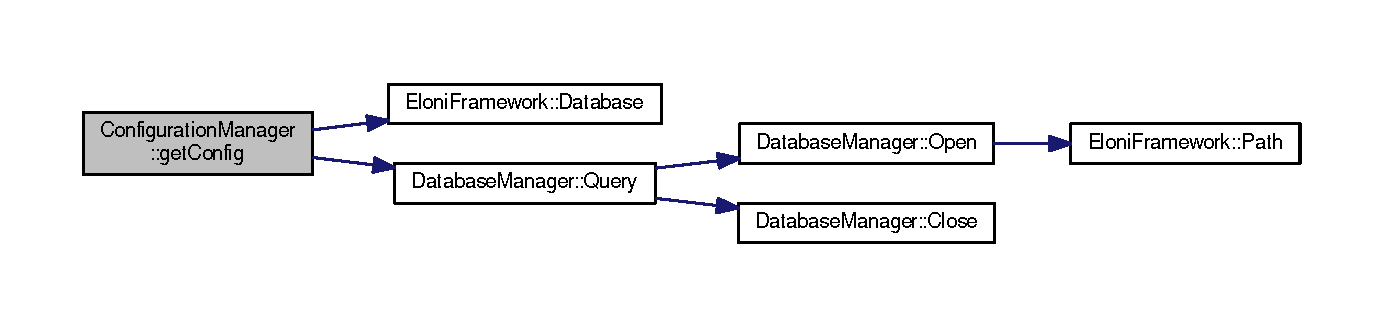
\includegraphics[width=350pt]{classConfigurationManager_ad3e85ee715420c432cd7545c6aaf8314_cgraph}
\end{center}
\end{figure}




The documentation for this class was generated from the following files\-:\begin{DoxyCompactItemize}
\item 
inc/\hyperlink{ConfigurationManager_8h}{Configuration\-Manager.\-h}\item 
src/Configuration\-Manager.\-cpp\end{DoxyCompactItemize}

\hypertarget{classDatabaseManager}{\section{Database\-Manager Class Reference}
\label{classDatabaseManager}\index{Database\-Manager@{Database\-Manager}}
}
\subsection*{Public Member Functions}
\begin{DoxyCompactItemize}
\item 
int \hyperlink{classDatabaseManager_a37b1f9148ca1b698c73a98bece97cd35}{Open} (std\-::string filename)
\begin{DoxyCompactList}\small\item\em Open the database. \end{DoxyCompactList}\item 
\hypertarget{classDatabaseManager_a5232ac6d9271e2b3984042c306157bdb}{void \hyperlink{classDatabaseManager_a5232ac6d9271e2b3984042c306157bdb}{Close} ()}\label{classDatabaseManager_a5232ac6d9271e2b3984042c306157bdb}

\begin{DoxyCompactList}\small\item\em Close the database. \end{DoxyCompactList}\item 
std\-::vector$<$ std\-::map\\*
$<$ std\-::string, std\-::string $>$ $>$ \hyperlink{classDatabaseManager_adefb1bdb51d7b23d4b3a446a3f22ea26}{Query} (std\-::string, std\-::string=\char`\"{}elonisas.\-db\char`\"{})
\begin{DoxyCompactList}\small\item\em Queries the database and returns the data in a dictionary style result for easy access (all values are fetched as string) \end{DoxyCompactList}\end{DoxyCompactItemize}


\subsection{Detailed Description}


Definition at line \hyperlink{DatabaseManager_8h_source_l00020}{20} of file \hyperlink{DatabaseManager_8h_source}{Database\-Manager.\-h}.



\subsection{Member Function Documentation}
\hypertarget{classDatabaseManager_a37b1f9148ca1b698c73a98bece97cd35}{\index{Database\-Manager@{Database\-Manager}!Open@{Open}}
\index{Open@{Open}!DatabaseManager@{Database\-Manager}}
\subsubsection[{Open}]{\setlength{\rightskip}{0pt plus 5cm}int Database\-Manager\-::\-Open (
\begin{DoxyParamCaption}
\item[{std\-::string}]{filename}
\end{DoxyParamCaption}
)}}\label{classDatabaseManager_a37b1f9148ca1b698c73a98bece97cd35}


Open the database. 

\begin{DoxyReturn}{Returns}
int 
\end{DoxyReturn}


Definition at line \hyperlink{DatabaseManager_8cpp_source_l00010}{10} of file \hyperlink{DatabaseManager_8cpp_source}{Database\-Manager.\-cpp}.



Here is the call graph for this function\-:
\nopagebreak
\begin{figure}[H]
\begin{center}
\leavevmode
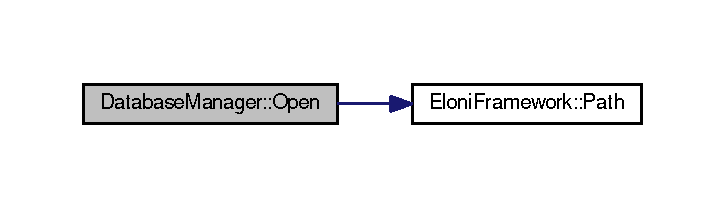
\includegraphics[width=348pt]{classDatabaseManager_a37b1f9148ca1b698c73a98bece97cd35_cgraph}
\end{center}
\end{figure}


\hypertarget{classDatabaseManager_adefb1bdb51d7b23d4b3a446a3f22ea26}{\index{Database\-Manager@{Database\-Manager}!Query@{Query}}
\index{Query@{Query}!DatabaseManager@{Database\-Manager}}
\subsubsection[{Query}]{\setlength{\rightskip}{0pt plus 5cm}std\-::vector$<$ std\-::map$<$ std\-::string, std\-::string $>$ $>$ Database\-Manager\-::\-Query (
\begin{DoxyParamCaption}
\item[{std\-::string}]{query, }
\item[{std\-::string}]{filename = {\ttfamily \char`\"{}elonisas.db\char`\"{}}}
\end{DoxyParamCaption}
)}}\label{classDatabaseManager_adefb1bdb51d7b23d4b3a446a3f22ea26}


Queries the database and returns the data in a dictionary style result for easy access (all values are fetched as string) 

eg\-: result\mbox{[}0\mbox{]}\mbox{[}\char`\"{}username\char`\"{}\mbox{]}

return vector$<$map$<$string, string$>$$>$ 

Definition at line \hyperlink{DatabaseManager_8cpp_source_l00038}{38} of file \hyperlink{DatabaseManager_8cpp_source}{Database\-Manager.\-cpp}.



Here is the call graph for this function\-:
\nopagebreak
\begin{figure}[H]
\begin{center}
\leavevmode
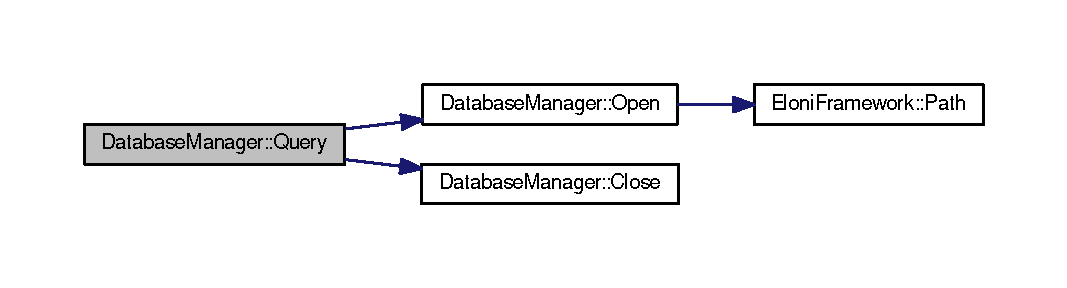
\includegraphics[width=350pt]{classDatabaseManager_adefb1bdb51d7b23d4b3a446a3f22ea26_cgraph}
\end{center}
\end{figure}




The documentation for this class was generated from the following files\-:\begin{DoxyCompactItemize}
\item 
inc/\hyperlink{DatabaseManager_8h}{Database\-Manager.\-h}\item 
src/Database\-Manager.\-cpp\end{DoxyCompactItemize}

\hypertarget{classEloniFramework}{\section{Eloni\-Framework Class Reference}
\label{classEloniFramework}\index{Eloni\-Framework@{Eloni\-Framework}}
}
\subsection*{Static Public Member Functions}
\begin{DoxyCompactItemize}
\item 
static \hyperlink{classDatabaseManager}{Database\-Manager} $\ast$ \hyperlink{classEloniFramework_a803da824e33d75564d5a7ca77e66b0e4}{Database} ()
\begin{DoxyCompactList}\small\item\em Returns the instance of \hyperlink{classDatabaseManager}{Database\-Manager}. \end{DoxyCompactList}\item 
static \hyperlink{classConfigurationManager}{Configuration\-Manager} $\ast$ \hyperlink{classEloniFramework_a3ef2e10a4eae52e233931cff12aadb48}{Configuration} ()
\begin{DoxyCompactList}\small\item\em Returns the instance of \hyperlink{classConfigurationManager}{Configuration\-Manager}. \end{DoxyCompactList}\item 
static \hyperlink{classSecurityManager}{Security\-Manager} $\ast$ \hyperlink{classEloniFramework_a417d0368e8e814f717a2b210496f7db2}{Security} ()
\begin{DoxyCompactList}\small\item\em Returns the instance of \hyperlink{classSecurityManager}{Security\-Manager}. \end{DoxyCompactList}\item 
static \hyperlink{classShellManager}{Shell\-Manager} $\ast$ \hyperlink{classEloniFramework_ac0bcb257424435f01d2da61a816db01a}{Shell} ()
\begin{DoxyCompactList}\small\item\em Returns the instance of \hyperlink{classShellManager}{Shell\-Manager}. \end{DoxyCompactList}\item 
static std\-::string \hyperlink{classEloniFramework_a97ba3c1e7eed84a52a572794c6f78eab}{Path} ()
\begin{DoxyCompactList}\small\item\em Returns the application directory. \end{DoxyCompactList}\end{DoxyCompactItemize}


\subsection{Detailed Description}


Definition at line \hyperlink{EloniFrameWork_8h_source_l00021}{21} of file \hyperlink{EloniFrameWork_8h_source}{Eloni\-Frame\-Work.\-h}.



\subsection{Member Function Documentation}
\hypertarget{classEloniFramework_a3ef2e10a4eae52e233931cff12aadb48}{\index{Eloni\-Framework@{Eloni\-Framework}!Configuration@{Configuration}}
\index{Configuration@{Configuration}!EloniFramework@{Eloni\-Framework}}
\subsubsection[{Configuration}]{\setlength{\rightskip}{0pt plus 5cm}{\bf Configuration\-Manager} $\ast$ Eloni\-Framework\-::\-Configuration (
\begin{DoxyParamCaption}
{}
\end{DoxyParamCaption}
)\hspace{0.3cm}{\ttfamily [static]}}}\label{classEloniFramework_a3ef2e10a4eae52e233931cff12aadb48}


Returns the instance of \hyperlink{classConfigurationManager}{Configuration\-Manager}. 

\begin{DoxyReturn}{Returns}
\hyperlink{classConfigurationManager}{Configuration\-Manager} 
\end{DoxyReturn}


Definition at line \hyperlink{EloniFrameWork_8cpp_source_l00013}{13} of file \hyperlink{EloniFrameWork_8cpp_source}{Eloni\-Frame\-Work.\-cpp}.

\hypertarget{classEloniFramework_a803da824e33d75564d5a7ca77e66b0e4}{\index{Eloni\-Framework@{Eloni\-Framework}!Database@{Database}}
\index{Database@{Database}!EloniFramework@{Eloni\-Framework}}
\subsubsection[{Database}]{\setlength{\rightskip}{0pt plus 5cm}{\bf Database\-Manager} $\ast$ Eloni\-Framework\-::\-Database (
\begin{DoxyParamCaption}
{}
\end{DoxyParamCaption}
)\hspace{0.3cm}{\ttfamily [static]}}}\label{classEloniFramework_a803da824e33d75564d5a7ca77e66b0e4}


Returns the instance of \hyperlink{classDatabaseManager}{Database\-Manager}. 

\begin{DoxyReturn}{Returns}
\hyperlink{classDatabaseManager}{Database\-Manager} 
\end{DoxyReturn}


Definition at line \hyperlink{EloniFrameWork_8cpp_source_l00025}{25} of file \hyperlink{EloniFrameWork_8cpp_source}{Eloni\-Frame\-Work.\-cpp}.

\hypertarget{classEloniFramework_a97ba3c1e7eed84a52a572794c6f78eab}{\index{Eloni\-Framework@{Eloni\-Framework}!Path@{Path}}
\index{Path@{Path}!EloniFramework@{Eloni\-Framework}}
\subsubsection[{Path}]{\setlength{\rightskip}{0pt plus 5cm}std\-::string Eloni\-Framework\-::\-Path (
\begin{DoxyParamCaption}
{}
\end{DoxyParamCaption}
)\hspace{0.3cm}{\ttfamily [static]}}}\label{classEloniFramework_a97ba3c1e7eed84a52a572794c6f78eab}


Returns the application directory. 

\begin{DoxyReturn}{Returns}
string 
\end{DoxyReturn}


Definition at line \hyperlink{EloniFrameWork_8cpp_source_l00061}{61} of file \hyperlink{EloniFrameWork_8cpp_source}{Eloni\-Frame\-Work.\-cpp}.

\hypertarget{classEloniFramework_a417d0368e8e814f717a2b210496f7db2}{\index{Eloni\-Framework@{Eloni\-Framework}!Security@{Security}}
\index{Security@{Security}!EloniFramework@{Eloni\-Framework}}
\subsubsection[{Security}]{\setlength{\rightskip}{0pt plus 5cm}{\bf Security\-Manager} $\ast$ Eloni\-Framework\-::\-Security (
\begin{DoxyParamCaption}
{}
\end{DoxyParamCaption}
)\hspace{0.3cm}{\ttfamily [static]}}}\label{classEloniFramework_a417d0368e8e814f717a2b210496f7db2}


Returns the instance of \hyperlink{classSecurityManager}{Security\-Manager}. 

\begin{DoxyReturn}{Returns}
\hyperlink{classSecurityManager}{Security\-Manager} 
\end{DoxyReturn}


Definition at line \hyperlink{EloniFrameWork_8cpp_source_l00037}{37} of file \hyperlink{EloniFrameWork_8cpp_source}{Eloni\-Frame\-Work.\-cpp}.

\hypertarget{classEloniFramework_ac0bcb257424435f01d2da61a816db01a}{\index{Eloni\-Framework@{Eloni\-Framework}!Shell@{Shell}}
\index{Shell@{Shell}!EloniFramework@{Eloni\-Framework}}
\subsubsection[{Shell}]{\setlength{\rightskip}{0pt plus 5cm}{\bf Shell\-Manager} $\ast$ Eloni\-Framework\-::\-Shell (
\begin{DoxyParamCaption}
{}
\end{DoxyParamCaption}
)\hspace{0.3cm}{\ttfamily [static]}}}\label{classEloniFramework_ac0bcb257424435f01d2da61a816db01a}


Returns the instance of \hyperlink{classShellManager}{Shell\-Manager}. 

\begin{DoxyReturn}{Returns}
\hyperlink{classShellManager}{Shell\-Manager} 
\end{DoxyReturn}


Definition at line \hyperlink{EloniFrameWork_8cpp_source_l00049}{49} of file \hyperlink{EloniFrameWork_8cpp_source}{Eloni\-Frame\-Work.\-cpp}.



The documentation for this class was generated from the following files\-:\begin{DoxyCompactItemize}
\item 
inc/Eloni\-Frame\-Work.\-h\item 
src/Eloni\-Frame\-Work.\-cpp\end{DoxyCompactItemize}

\hypertarget{classSecurityManager}{\section{Security\-Manager Class Reference}
\label{classSecurityManager}\index{Security\-Manager@{Security\-Manager}}
}
\subsection*{Public Member Functions}
\begin{DoxyCompactItemize}
\item 
std\-::string \hyperlink{classSecurityManager_acc4ef8e7685038735e83e73556a5f510}{Encrypt} (std\-::string str)
\begin{DoxyCompactList}\small\item\em Encrypt a string in D\-G Standard encryption. \end{DoxyCompactList}\item 
std\-::map$<$ std\-::string, int $>$ \hyperlink{classSecurityManager_afe3d50265be58ec179058feadd9902a6}{get\-Roles} ()
\begin{DoxyCompactList}\small\item\em Get all roles from the database. \end{DoxyCompactList}\item 
bool \hyperlink{classSecurityManager_a2950edc6463999ceca399d47023adddc}{has\-Role} (std\-::string username, std\-::string role)
\begin{DoxyCompactList}\small\item\em Check if a user has a specific role. \end{DoxyCompactList}\item 
\hypertarget{classSecurityManager_a9ebf385f13f1893bb36647605677043d}{void \hyperlink{classSecurityManager_a9ebf385f13f1893bb36647605677043d}{add\-Role} (std\-::string username, std\-::string role)}\label{classSecurityManager_a9ebf385f13f1893bb36647605677043d}

\begin{DoxyCompactList}\small\item\em Assign a role to a user. \end{DoxyCompactList}\item 
\hypertarget{classSecurityManager_a2d5b4923acbe73b0d21c5179deb7f17d}{void \hyperlink{classSecurityManager_a2d5b4923acbe73b0d21c5179deb7f17d}{remove\-Role} (std\-::string username, std\-::string role)}\label{classSecurityManager_a2d5b4923acbe73b0d21c5179deb7f17d}

\begin{DoxyCompactList}\small\item\em Remove a role from a user. \end{DoxyCompactList}\item 
\hypertarget{classSecurityManager_ac9dc2c5a7667b95d9850ff22fc897213}{void \hyperlink{classSecurityManager_ac9dc2c5a7667b95d9850ff22fc897213}{add\-User} (std\-::string username, std\-::string password)}\label{classSecurityManager_ac9dc2c5a7667b95d9850ff22fc897213}

\begin{DoxyCompactList}\small\item\em Add a user. \end{DoxyCompactList}\item 
\hypertarget{classSecurityManager_ad616d32abdd366d50dfd01091d6a1f0c}{void \hyperlink{classSecurityManager_ad616d32abdd366d50dfd01091d6a1f0c}{set\-User} (std\-::string username, std\-::string var, std\-::string val)}\label{classSecurityManager_ad616d32abdd366d50dfd01091d6a1f0c}

\begin{DoxyCompactList}\small\item\em Set user properties. \end{DoxyCompactList}\item 
\hypertarget{classSecurityManager_a61db3bbbb21105c441d2a7bc75fb41bd}{void \hyperlink{classSecurityManager_a61db3bbbb21105c441d2a7bc75fb41bd}{delete\-User} (std\-::string username)}\label{classSecurityManager_a61db3bbbb21105c441d2a7bc75fb41bd}

\begin{DoxyCompactList}\small\item\em Remove a user. \end{DoxyCompactList}\item 
bool \hyperlink{classSecurityManager_abda859f83e39977a46ce993970a35f92}{is\-User} (std\-::string username)
\begin{DoxyCompactList}\small\item\em Check if a user exists. \end{DoxyCompactList}\item 
std\-::vector$<$ std\-::string $>$ \hyperlink{classSecurityManager_a05f3c7fc498871277a00dffa092614c1}{get\-Users} ()
\begin{DoxyCompactList}\small\item\em Get all users from the database. \end{DoxyCompactList}\item 
bool \hyperlink{classSecurityManager_ace68188567f645c18097b8791db64b41}{Authenticate} (std\-::string username, std\-::string password)
\begin{DoxyCompactList}\small\item\em Authenticate a uer. \end{DoxyCompactList}\end{DoxyCompactItemize}


\subsection{Detailed Description}


Definition at line \hyperlink{SecurityManager_8h_source_l00023}{23} of file \hyperlink{SecurityManager_8h_source}{Security\-Manager.\-h}.



\subsection{Member Function Documentation}
\hypertarget{classSecurityManager_ace68188567f645c18097b8791db64b41}{\index{Security\-Manager@{Security\-Manager}!Authenticate@{Authenticate}}
\index{Authenticate@{Authenticate}!SecurityManager@{Security\-Manager}}
\subsubsection[{Authenticate}]{\setlength{\rightskip}{0pt plus 5cm}bool Security\-Manager\-::\-Authenticate (
\begin{DoxyParamCaption}
\item[{std\-::string}]{username, }
\item[{std\-::string}]{password}
\end{DoxyParamCaption}
)}}\label{classSecurityManager_ace68188567f645c18097b8791db64b41}


Authenticate a uer. 

\begin{DoxyReturn}{Returns}
bool 
\end{DoxyReturn}


Definition at line \hyperlink{SecurityManager_8cpp_source_l00129}{129} of file \hyperlink{SecurityManager_8cpp_source}{Security\-Manager.\-cpp}.



Here is the call graph for this function\-:
\nopagebreak
\begin{figure}[H]
\begin{center}
\leavevmode
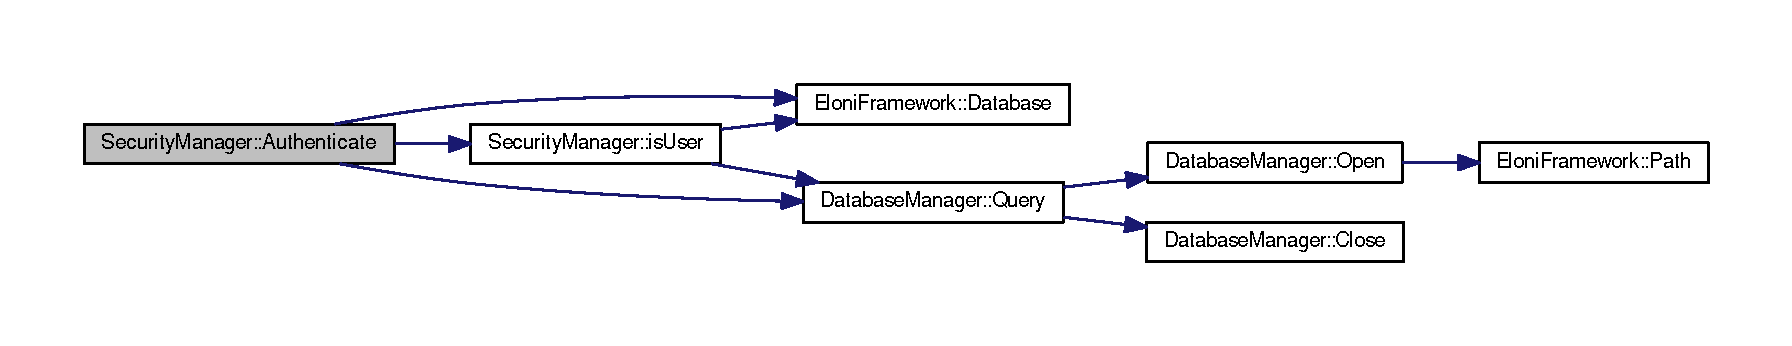
\includegraphics[width=350pt]{classSecurityManager_ace68188567f645c18097b8791db64b41_cgraph}
\end{center}
\end{figure}


\hypertarget{classSecurityManager_acc4ef8e7685038735e83e73556a5f510}{\index{Security\-Manager@{Security\-Manager}!Encrypt@{Encrypt}}
\index{Encrypt@{Encrypt}!SecurityManager@{Security\-Manager}}
\subsubsection[{Encrypt}]{\setlength{\rightskip}{0pt plus 5cm}std\-::string Security\-Manager\-::\-Encrypt (
\begin{DoxyParamCaption}
\item[{std\-::string}]{str}
\end{DoxyParamCaption}
)}}\label{classSecurityManager_acc4ef8e7685038735e83e73556a5f510}


Encrypt a string in D\-G Standard encryption. 

\begin{DoxyReturn}{Returns}
string 
\end{DoxyReturn}


Definition at line \hyperlink{SecurityManager_8cpp_source_l00008}{8} of file \hyperlink{SecurityManager_8cpp_source}{Security\-Manager.\-cpp}.

\hypertarget{classSecurityManager_afe3d50265be58ec179058feadd9902a6}{\index{Security\-Manager@{Security\-Manager}!get\-Roles@{get\-Roles}}
\index{get\-Roles@{get\-Roles}!SecurityManager@{Security\-Manager}}
\subsubsection[{get\-Roles}]{\setlength{\rightskip}{0pt plus 5cm}std\-::map$<$ std\-::string, int $>$ Security\-Manager\-::get\-Roles (
\begin{DoxyParamCaption}
{}
\end{DoxyParamCaption}
)}}\label{classSecurityManager_afe3d50265be58ec179058feadd9902a6}


Get all roles from the database. 

\begin{DoxyReturn}{Returns}
std\-::map$<$std\-::string, int$>$ 
\end{DoxyReturn}


Definition at line \hyperlink{SecurityManager_8cpp_source_l00076}{76} of file \hyperlink{SecurityManager_8cpp_source}{Security\-Manager.\-cpp}.



Here is the call graph for this function\-:
\nopagebreak
\begin{figure}[H]
\begin{center}
\leavevmode
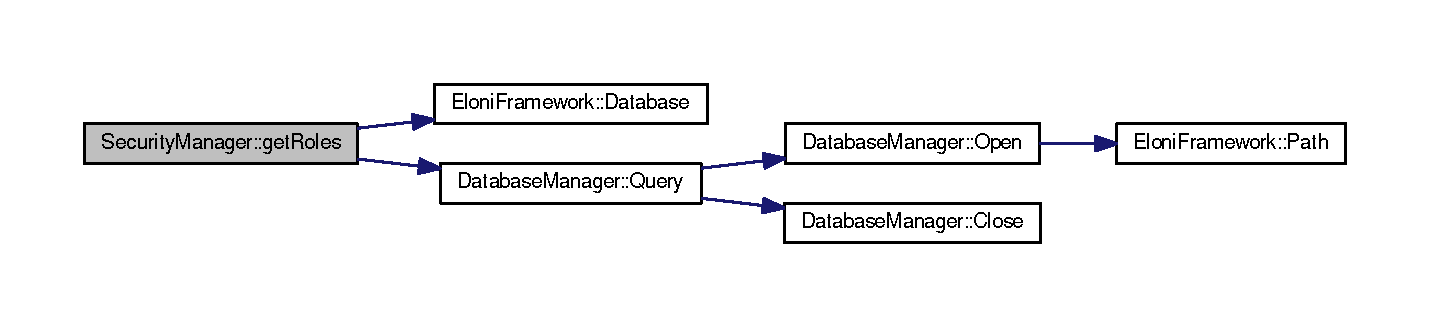
\includegraphics[width=350pt]{classSecurityManager_afe3d50265be58ec179058feadd9902a6_cgraph}
\end{center}
\end{figure}


\hypertarget{classSecurityManager_a05f3c7fc498871277a00dffa092614c1}{\index{Security\-Manager@{Security\-Manager}!get\-Users@{get\-Users}}
\index{get\-Users@{get\-Users}!SecurityManager@{Security\-Manager}}
\subsubsection[{get\-Users}]{\setlength{\rightskip}{0pt plus 5cm}std\-::vector$<$ std\-::string $>$ Security\-Manager\-::get\-Users (
\begin{DoxyParamCaption}
{}
\end{DoxyParamCaption}
)}}\label{classSecurityManager_a05f3c7fc498871277a00dffa092614c1}


Get all users from the database. 

\begin{DoxyReturn}{Returns}
std\-::vector 
\end{DoxyReturn}


Definition at line \hyperlink{SecurityManager_8cpp_source_l00060}{60} of file \hyperlink{SecurityManager_8cpp_source}{Security\-Manager.\-cpp}.



Here is the call graph for this function\-:
\nopagebreak
\begin{figure}[H]
\begin{center}
\leavevmode
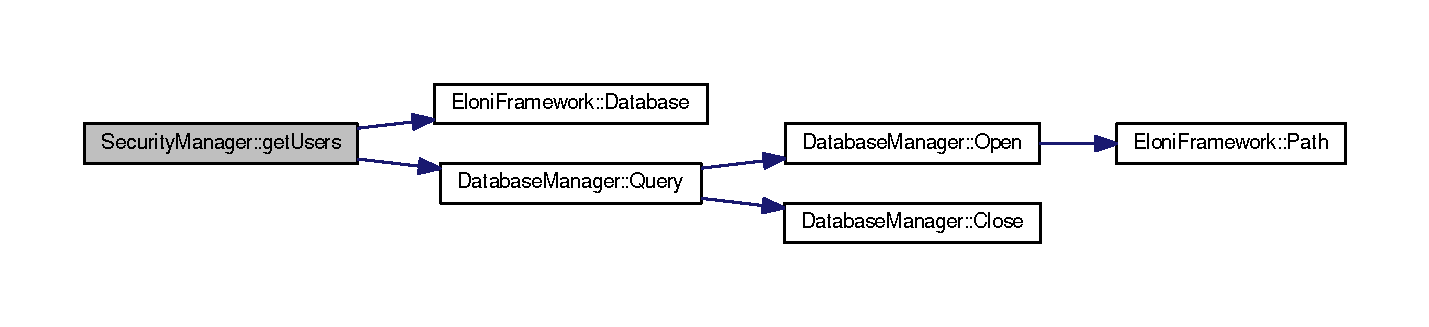
\includegraphics[width=350pt]{classSecurityManager_a05f3c7fc498871277a00dffa092614c1_cgraph}
\end{center}
\end{figure}


\hypertarget{classSecurityManager_a2950edc6463999ceca399d47023adddc}{\index{Security\-Manager@{Security\-Manager}!has\-Role@{has\-Role}}
\index{has\-Role@{has\-Role}!SecurityManager@{Security\-Manager}}
\subsubsection[{has\-Role}]{\setlength{\rightskip}{0pt plus 5cm}bool Security\-Manager\-::has\-Role (
\begin{DoxyParamCaption}
\item[{std\-::string}]{username, }
\item[{std\-::string}]{role}
\end{DoxyParamCaption}
)}}\label{classSecurityManager_a2950edc6463999ceca399d47023adddc}


Check if a user has a specific role. 

\begin{DoxyReturn}{Returns}
bool 
\end{DoxyReturn}


Definition at line \hyperlink{SecurityManager_8cpp_source_l00092}{92} of file \hyperlink{SecurityManager_8cpp_source}{Security\-Manager.\-cpp}.



Here is the call graph for this function\-:
\nopagebreak
\begin{figure}[H]
\begin{center}
\leavevmode
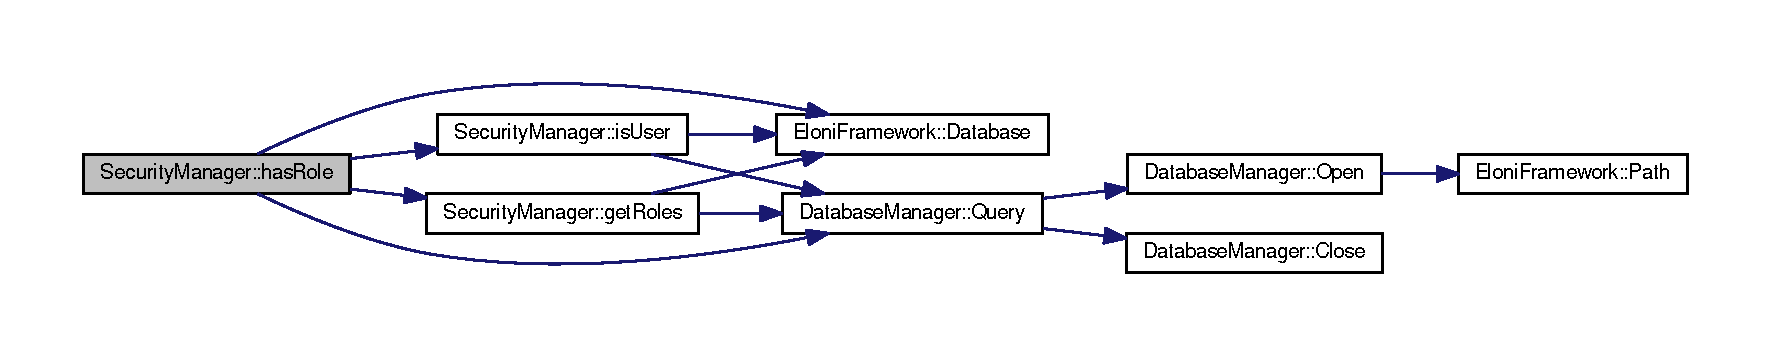
\includegraphics[width=350pt]{classSecurityManager_a2950edc6463999ceca399d47023adddc_cgraph}
\end{center}
\end{figure}


\hypertarget{classSecurityManager_abda859f83e39977a46ce993970a35f92}{\index{Security\-Manager@{Security\-Manager}!is\-User@{is\-User}}
\index{is\-User@{is\-User}!SecurityManager@{Security\-Manager}}
\subsubsection[{is\-User}]{\setlength{\rightskip}{0pt plus 5cm}bool Security\-Manager\-::is\-User (
\begin{DoxyParamCaption}
\item[{std\-::string}]{username}
\end{DoxyParamCaption}
)}}\label{classSecurityManager_abda859f83e39977a46ce993970a35f92}


Check if a user exists. 

\begin{DoxyReturn}{Returns}
bool 
\end{DoxyReturn}


Definition at line \hyperlink{SecurityManager_8cpp_source_l00047}{47} of file \hyperlink{SecurityManager_8cpp_source}{Security\-Manager.\-cpp}.



Here is the call graph for this function\-:
\nopagebreak
\begin{figure}[H]
\begin{center}
\leavevmode
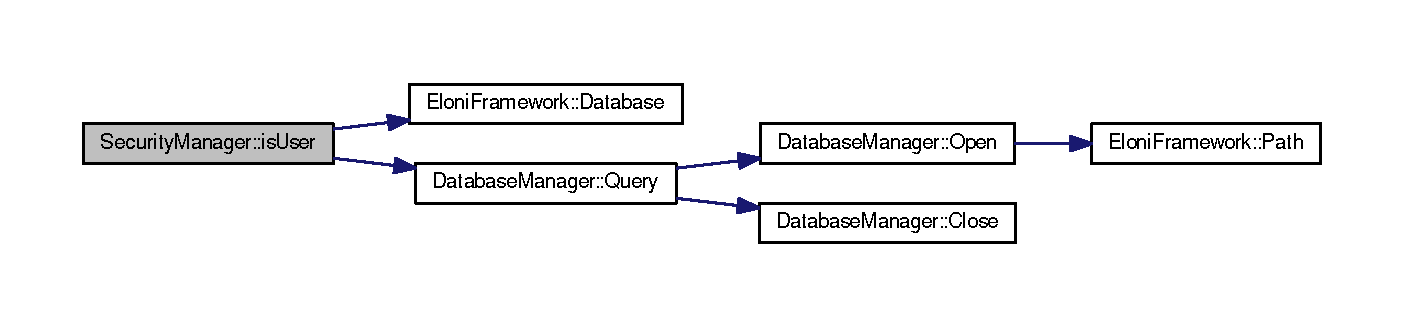
\includegraphics[width=350pt]{classSecurityManager_abda859f83e39977a46ce993970a35f92_cgraph}
\end{center}
\end{figure}




The documentation for this class was generated from the following files\-:\begin{DoxyCompactItemize}
\item 
inc/\hyperlink{SecurityManager_8h}{Security\-Manager.\-h}\item 
src/Security\-Manager.\-cpp\end{DoxyCompactItemize}

\hypertarget{classShellManager}{\section{Shell\-Manager Class Reference}
\label{classShellManager}\index{Shell\-Manager@{Shell\-Manager}}
}
\subsection*{Public Member Functions}
\begin{DoxyCompactItemize}
\item 
\hyperlink{classShellManager_a04dec3699269bb388648f6017fd9fd15}{Shell\-Manager} ()
\begin{DoxyCompactList}\small\item\em Constructor. \end{DoxyCompactList}\item 
int \hyperlink{classShellManager_a9e595c79f89d7c796df213b469384e08}{set\-User} (std\-::string Username)
\begin{DoxyCompactList}\small\item\em Attempt to set the user id based on username. \end{DoxyCompactList}\item 
int \hyperlink{classShellManager_a0451c163858db5c51c8976d9bf7dd37d}{set\-User} (int User\-I\-D)
\begin{DoxyCompactList}\small\item\em Set active userid. \end{DoxyCompactList}\item 
std\-::string \hyperlink{classShellManager_aeed1b234a317e951f01bdc42a2097d40}{set\-Working\-Directory} (std\-::string dir)
\begin{DoxyCompactList}\small\item\em Set working directory. \end{DoxyCompactList}\item 
std\-::string \hyperlink{classShellManager_a9f40b1296bef8f0d694cafdca29e0e13}{Execute} (std\-::string cmd)
\begin{DoxyCompactList}\small\item\em Execute a bash command in working directory. \end{DoxyCompactList}\end{DoxyCompactItemize}


\subsection{Detailed Description}


Definition at line \hyperlink{ShellManager_8h_source_l00025}{25} of file \hyperlink{ShellManager_8h_source}{Shell\-Manager.\-h}.



\subsection{Constructor \& Destructor Documentation}
\hypertarget{classShellManager_a04dec3699269bb388648f6017fd9fd15}{\index{Shell\-Manager@{Shell\-Manager}!Shell\-Manager@{Shell\-Manager}}
\index{Shell\-Manager@{Shell\-Manager}!ShellManager@{Shell\-Manager}}
\subsubsection[{Shell\-Manager}]{\setlength{\rightskip}{0pt plus 5cm}Shell\-Manager\-::\-Shell\-Manager (
\begin{DoxyParamCaption}
{}
\end{DoxyParamCaption}
)}}\label{classShellManager_a04dec3699269bb388648f6017fd9fd15}


Constructor. 

Fill the blacklist 

Definition at line \hyperlink{ShellManager_8cpp_source_l00008}{8} of file \hyperlink{ShellManager_8cpp_source}{Shell\-Manager.\-cpp}.



\subsection{Member Function Documentation}
\hypertarget{classShellManager_a9f40b1296bef8f0d694cafdca29e0e13}{\index{Shell\-Manager@{Shell\-Manager}!Execute@{Execute}}
\index{Execute@{Execute}!ShellManager@{Shell\-Manager}}
\subsubsection[{Execute}]{\setlength{\rightskip}{0pt plus 5cm}std\-::string Shell\-Manager\-::\-Execute (
\begin{DoxyParamCaption}
\item[{std\-::string}]{cmd}
\end{DoxyParamCaption}
)}}\label{classShellManager_a9f40b1296bef8f0d694cafdca29e0e13}


Execute a bash command in working directory. 

\begin{DoxyReturn}{Returns}
string bash output 
\end{DoxyReturn}


Definition at line \hyperlink{ShellManager_8cpp_source_l00080}{80} of file \hyperlink{ShellManager_8cpp_source}{Shell\-Manager.\-cpp}.

\hypertarget{classShellManager_a9e595c79f89d7c796df213b469384e08}{\index{Shell\-Manager@{Shell\-Manager}!set\-User@{set\-User}}
\index{set\-User@{set\-User}!ShellManager@{Shell\-Manager}}
\subsubsection[{set\-User}]{\setlength{\rightskip}{0pt plus 5cm}int Shell\-Manager\-::set\-User (
\begin{DoxyParamCaption}
\item[{std\-::string}]{Username}
\end{DoxyParamCaption}
)}}\label{classShellManager_a9e595c79f89d7c796df213b469384e08}


Attempt to set the user id based on username. 

\begin{DoxyReturn}{Returns}
int 
\end{DoxyReturn}


Definition at line \hyperlink{ShellManager_8cpp_source_l00022}{22} of file \hyperlink{ShellManager_8cpp_source}{Shell\-Manager.\-cpp}.

\hypertarget{classShellManager_a0451c163858db5c51c8976d9bf7dd37d}{\index{Shell\-Manager@{Shell\-Manager}!set\-User@{set\-User}}
\index{set\-User@{set\-User}!ShellManager@{Shell\-Manager}}
\subsubsection[{set\-User}]{\setlength{\rightskip}{0pt plus 5cm}int Shell\-Manager\-::set\-User (
\begin{DoxyParamCaption}
\item[{int}]{User\-I\-D}
\end{DoxyParamCaption}
)}}\label{classShellManager_a0451c163858db5c51c8976d9bf7dd37d}


Set active userid. 

\begin{DoxyReturn}{Returns}
int setresuid 
\end{DoxyReturn}


Definition at line \hyperlink{ShellManager_8cpp_source_l00053}{53} of file \hyperlink{ShellManager_8cpp_source}{Shell\-Manager.\-cpp}.

\hypertarget{classShellManager_aeed1b234a317e951f01bdc42a2097d40}{\index{Shell\-Manager@{Shell\-Manager}!set\-Working\-Directory@{set\-Working\-Directory}}
\index{set\-Working\-Directory@{set\-Working\-Directory}!ShellManager@{Shell\-Manager}}
\subsubsection[{set\-Working\-Directory}]{\setlength{\rightskip}{0pt plus 5cm}std\-::string Shell\-Manager\-::set\-Working\-Directory (
\begin{DoxyParamCaption}
\item[{std\-::string}]{dir}
\end{DoxyParamCaption}
)}}\label{classShellManager_aeed1b234a317e951f01bdc42a2097d40}


Set working directory. 

\begin{DoxyReturn}{Returns}
string working directory or application binary directory if fail 
\end{DoxyReturn}


Definition at line \hyperlink{ShellManager_8cpp_source_l00064}{64} of file \hyperlink{ShellManager_8cpp_source}{Shell\-Manager.\-cpp}.



Here is the call graph for this function\-:
\nopagebreak
\begin{figure}[H]
\begin{center}
\leavevmode
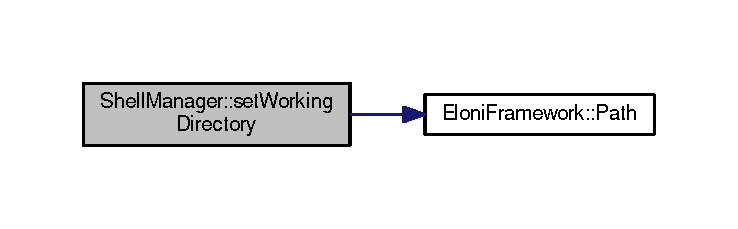
\includegraphics[width=350pt]{classShellManager_aeed1b234a317e951f01bdc42a2097d40_cgraph}
\end{center}
\end{figure}




The documentation for this class was generated from the following files\-:\begin{DoxyCompactItemize}
\item 
inc/\hyperlink{ShellManager_8h}{Shell\-Manager.\-h}\item 
src/Shell\-Manager.\-cpp\end{DoxyCompactItemize}

\chapter{File Documentation}
\hypertarget{ConfigurationManager_8h}{\section{inc/\-Configuration\-Manager.h File Reference}
\label{ConfigurationManager_8h}\index{inc/\-Configuration\-Manager.\-h@{inc/\-Configuration\-Manager.\-h}}
}
{\ttfamily \#include \char`\"{}Includes.\-h\char`\"{}}\\*
Include dependency graph for Configuration\-Manager.\-h\-:
\nopagebreak
\begin{figure}[H]
\begin{center}
\leavevmode
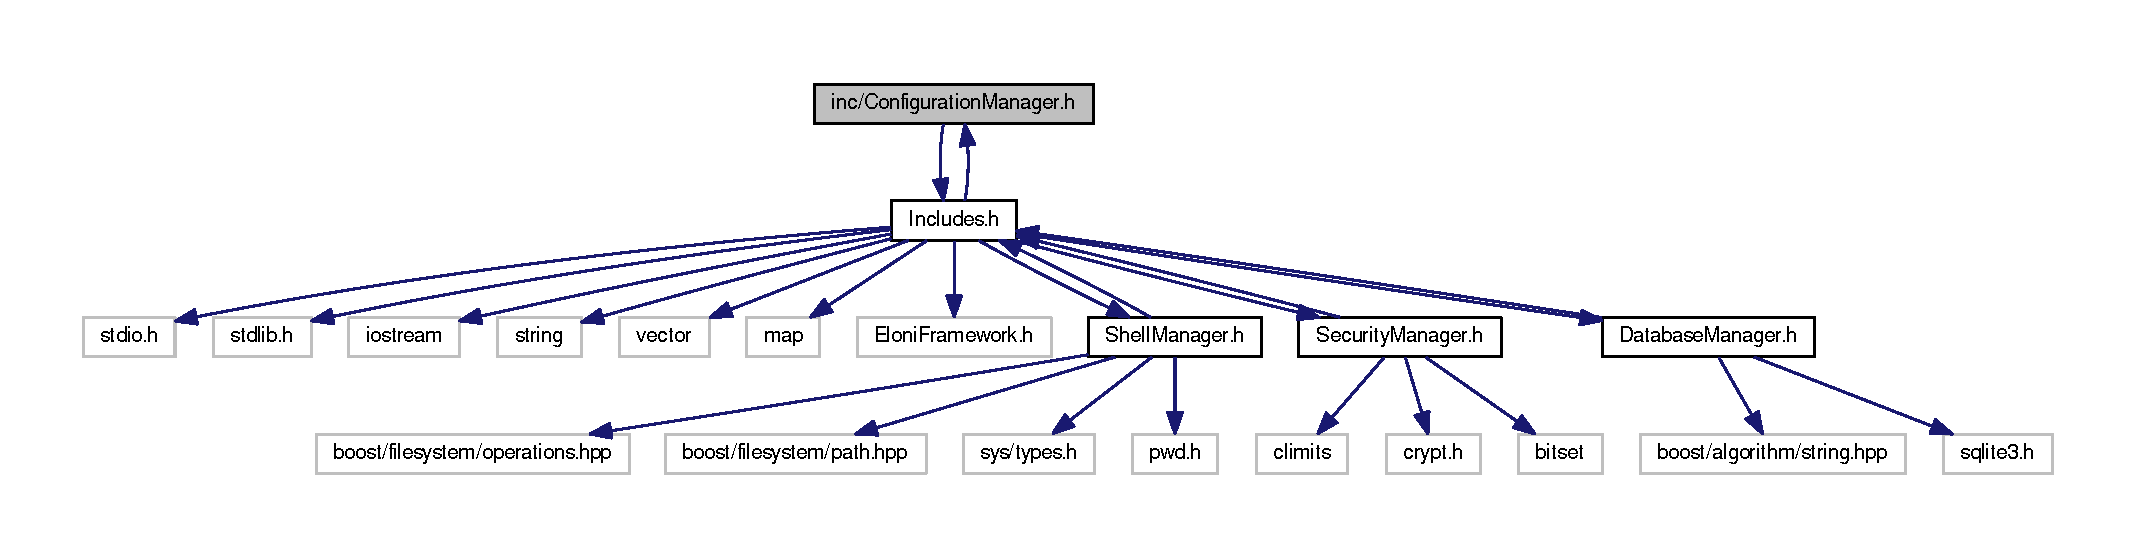
\includegraphics[width=350pt]{ConfigurationManager_8h__incl}
\end{center}
\end{figure}
This graph shows which files directly or indirectly include this file\-:
\nopagebreak
\begin{figure}[H]
\begin{center}
\leavevmode
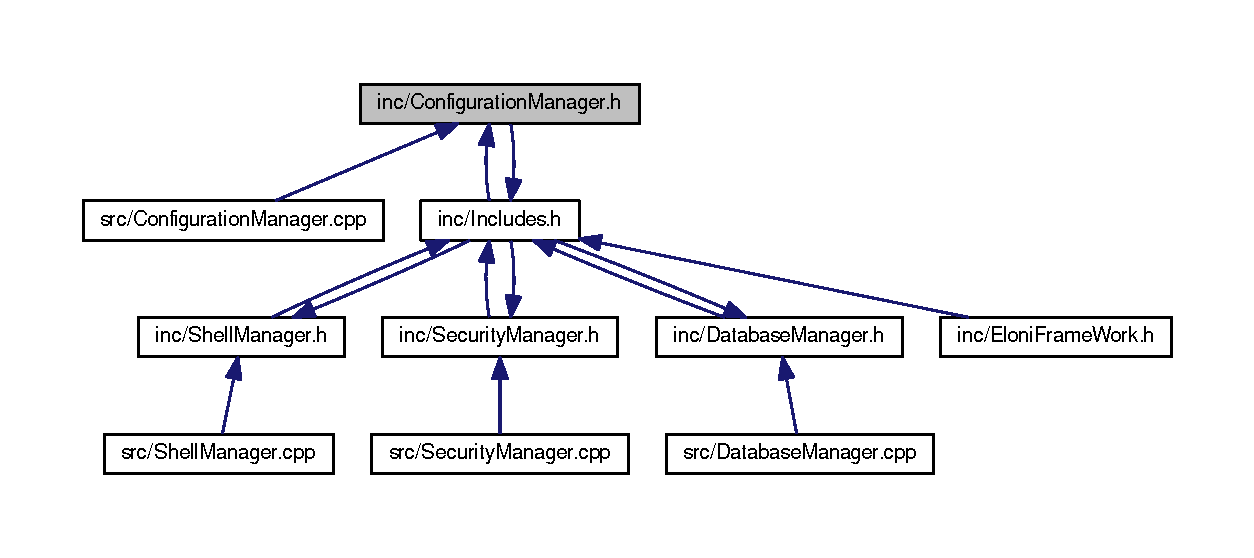
\includegraphics[width=350pt]{ConfigurationManager_8h__dep__incl}
\end{center}
\end{figure}
\subsection*{Classes}
\begin{DoxyCompactItemize}
\item 
class \hyperlink{classConfigurationManager}{Configuration\-Manager}
\end{DoxyCompactItemize}


\subsection{Detailed Description}
\begin{DoxyAuthor}{Author}
Yme-\/\-Jan Iedema \href{mailto:yj.iedema@gmail.com}{\tt yj.\-iedema@gmail.\-com}
\end{DoxyAuthor}
\hyperlink{classDatabaseManager}{Database\-Manager}

\hyperlink{classConfigurationManager}{Configuration\-Manager}

The configuration manager for getting configuration variables from and to the database 

Definition in file \hyperlink{ConfigurationManager_8h_source}{Configuration\-Manager.\-h}.


\hypertarget{ConfigurationManager_8h}{\section{Configuration\-Manager.\-h}
\label{ConfigurationManager_8h}\index{inc/\-Configuration\-Manager.\-h@{inc/\-Configuration\-Manager.\-h}}
}

\begin{DoxyCode}
00001 \textcolor{comment}{/**}
00002 \textcolor{comment}{ * @author Yme-Jan Iedema <yj.iedema@gmail.com>}
00003 \textcolor{comment}{ * @file ConfigurationManager.h}
00004 \textcolor{comment}{ * @dependency DatabaseManager}
00005 \textcolor{comment}{ * }
00006 \textcolor{comment}{ * ConfigurationManager}
00007 \textcolor{comment}{ * }
00008 \textcolor{comment}{ * The configuration manager for getting configuration variables from}
00009 \textcolor{comment}{ * and to the database}
00010 \textcolor{comment}{ */}
00011  
00012  
00013 \textcolor{preprocessor}{#ifndef DG2\_CONFIGURATIONMANAGER\_H}
00014 \textcolor{preprocessor}{}\textcolor{preprocessor}{#define DG2\_CONFIGURATIONMANAGER\_H}
00015 \textcolor{preprocessor}{}
00016 \textcolor{preprocessor}{#include "Includes.h"}
00017 
\hypertarget{ConfigurationManager_8h_source_l00018}{}\hyperlink{classConfigurationManager}{00018} \textcolor{keyword}{class }\hyperlink{classConfigurationManager}{ConfigurationManager} \{
00019   \textcolor{keyword}{private}:
00020     
00021   \textcolor{keyword}{public}:
00022     std::string \hyperlink{classConfigurationManager_ad3e85ee715420c432cd7545c6aaf8314}{getConfig}(std::string var);
00023     \textcolor{keywordtype}{void} \hyperlink{classConfigurationManager_ad027e09a69a516f2ad020c9cbdf49f2f}{setConfig}(std::string var, std::string val);
00024 \};
00025 
00026 \textcolor{preprocessor}{#endif}
\end{DoxyCode}

\hypertarget{DatabaseManager_8h}{\section{inc/\-Database\-Manager.h File Reference}
\label{DatabaseManager_8h}\index{inc/\-Database\-Manager.\-h@{inc/\-Database\-Manager.\-h}}
}
{\ttfamily \#include \char`\"{}Includes.\-h\char`\"{}}\\*
{\ttfamily \#include $<$boost/algorithm/string.\-hpp$>$}\\*
{\ttfamily \#include $<$sqlite3.\-h$>$}\\*
Include dependency graph for Database\-Manager.\-h\-:
\nopagebreak
\begin{figure}[H]
\begin{center}
\leavevmode
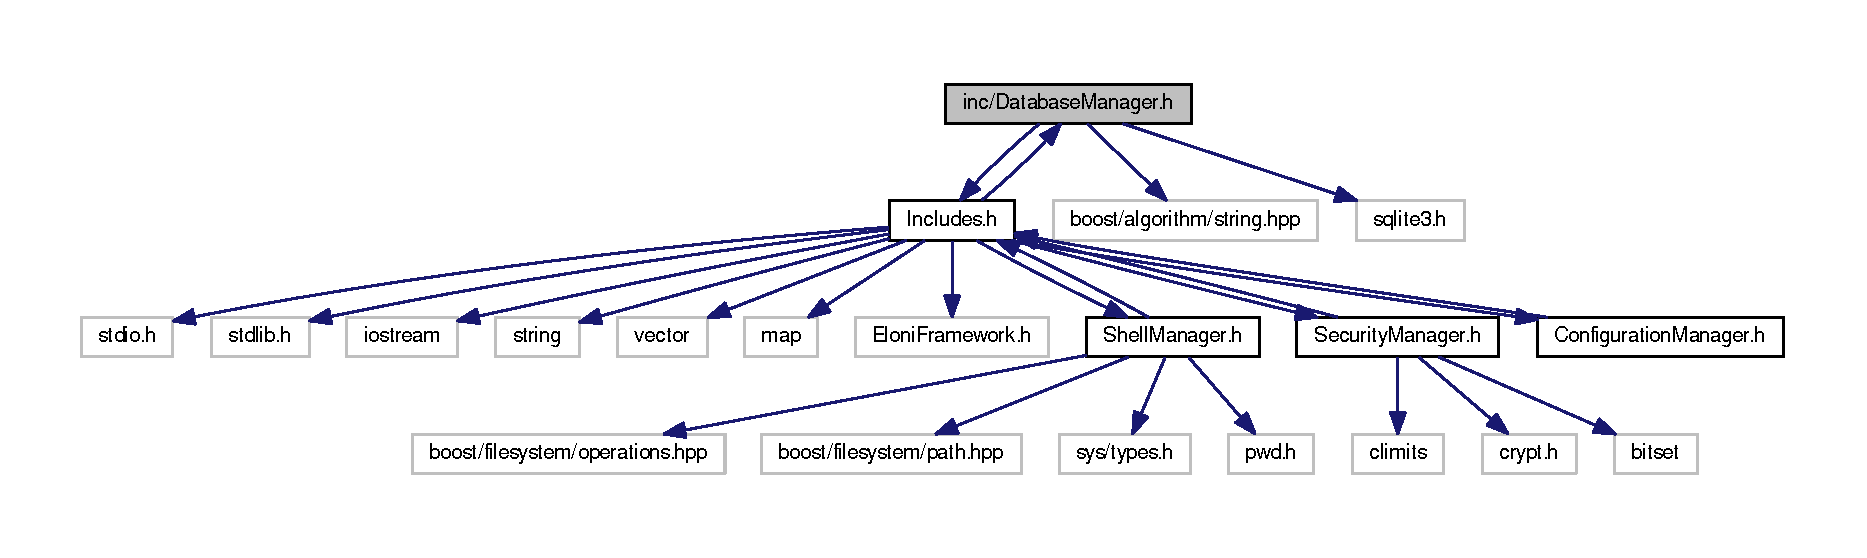
\includegraphics[width=350pt]{DatabaseManager_8h__incl}
\end{center}
\end{figure}
This graph shows which files directly or indirectly include this file\-:
\nopagebreak
\begin{figure}[H]
\begin{center}
\leavevmode
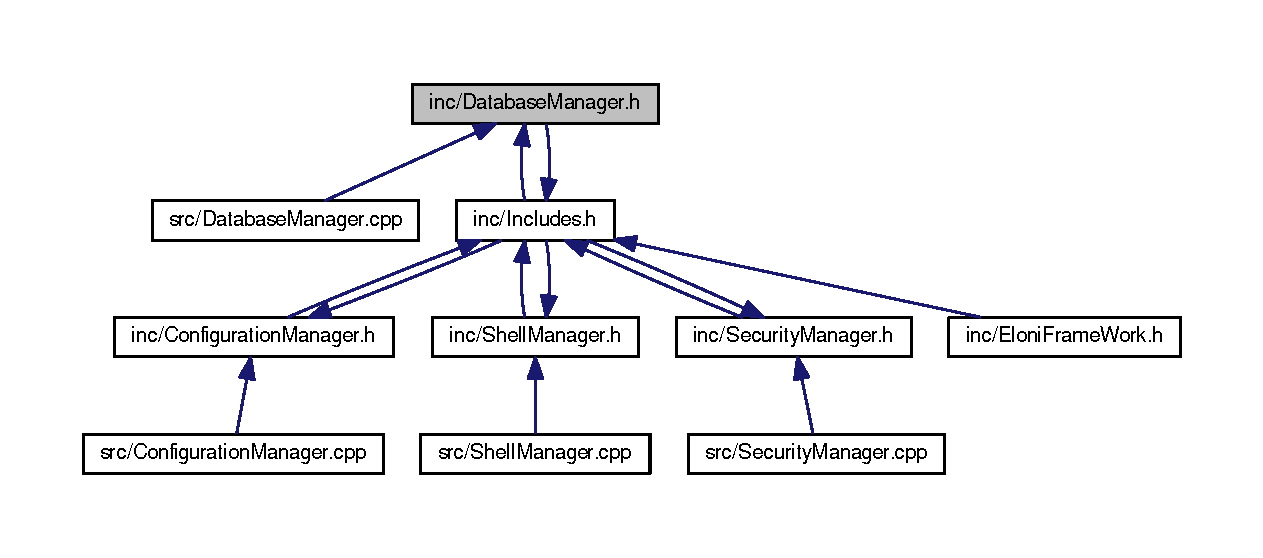
\includegraphics[width=350pt]{DatabaseManager_8h__dep__incl}
\end{center}
\end{figure}
\subsection*{Classes}
\begin{DoxyCompactItemize}
\item 
class \hyperlink{classDatabaseManager}{Database\-Manager}
\end{DoxyCompactItemize}


\subsection{Detailed Description}
\begin{DoxyAuthor}{Author}
Yme-\/\-Jan Iedema \href{mailto:yj.iedema@gmail.com}{\tt yj.\-iedema@gmail.\-com}
\end{DoxyAuthor}
\hyperlink{classDatabaseManager}{Database\-Manager}

Wrapper for sqlite The Query function throws a segementation error when accessing tables or data that does not exit 

Definition in file \hyperlink{DatabaseManager_8h_source}{Database\-Manager.\-h}.


\hypertarget{DatabaseManager_8h}{\section{Database\-Manager.\-h}
\label{DatabaseManager_8h}\index{inc/\-Database\-Manager.\-h@{inc/\-Database\-Manager.\-h}}
}

\begin{DoxyCode}
00001 \textcolor{comment}{/*!}
00002 \textcolor{comment}{ * @author Yme-Jan Iedema <yj.iedema@gmail.com>}
00003 \textcolor{comment}{ * @file DatabaseManager.h}
00004 \textcolor{comment}{ * }
00005 \textcolor{comment}{ * DatabaseManager}
00006 \textcolor{comment}{ * }
00007 \textcolor{comment}{ * Wrapper for sqlite}
00008 \textcolor{comment}{ * The Query function throws a segementation error when accessing}
00009 \textcolor{comment}{ * tables or data that does not exit}
00010 \textcolor{comment}{ */}
00011 
00012 \textcolor{preprocessor}{#ifndef DG2\_DATABASEMANAGER\_H}
00013 \textcolor{preprocessor}{}\textcolor{preprocessor}{#define DG2\_DATABASEMANAGER\_H}
00014 \textcolor{preprocessor}{}
00015 \textcolor{preprocessor}{#include "Includes.h"}
00016 
00017 \textcolor{preprocessor}{#include <boost/algorithm/string.hpp>}
00018 \textcolor{preprocessor}{#include <sqlite3.h>}
00019 
\hypertarget{DatabaseManager_8h_source_l00020}{}\hyperlink{classDatabaseManager}{00020} \textcolor{keyword}{class }\hyperlink{classDatabaseManager}{DatabaseManager} \{
00021   \textcolor{keyword}{private}:
00022     sqlite3     *db;
00023     \textcolor{keywordtype}{int}         rc;
00024     std::string dbFile;
00025     
00026   \textcolor{keyword}{public}:
00027     \hyperlink{classDatabaseManager}{DatabaseManager}();
00028     \textcolor{keywordtype}{int}           \hyperlink{classDatabaseManager_a37b1f9148ca1b698c73a98bece97cd35}{Open}(std::string filename);
00029     \textcolor{keywordtype}{void}          \hyperlink{classDatabaseManager_a5232ac6d9271e2b3984042c306157bdb}{Close}();
00030     std::vector< std::map<std::string,std::string> > \hyperlink{classDatabaseManager_adefb1bdb51d7b23d4b3a446a3f22ea26}{Query}(std::string, std::string = \textcolor{stringliteral}{"elonisas.db"});
00031     
00032 \};
00033 
00034 \textcolor{preprocessor}{#endif}
\end{DoxyCode}

\hypertarget{SecurityManager_8h}{\section{inc/\-Security\-Manager.h File Reference}
\label{SecurityManager_8h}\index{inc/\-Security\-Manager.\-h@{inc/\-Security\-Manager.\-h}}
}
{\ttfamily \#include \char`\"{}Includes.\-h\char`\"{}}\\*
{\ttfamily \#include $<$climits$>$}\\*
{\ttfamily \#include $<$crypt.\-h$>$}\\*
{\ttfamily \#include $<$bitset$>$}\\*
Include dependency graph for Security\-Manager.\-h\-:
\nopagebreak
\begin{figure}[H]
\begin{center}
\leavevmode
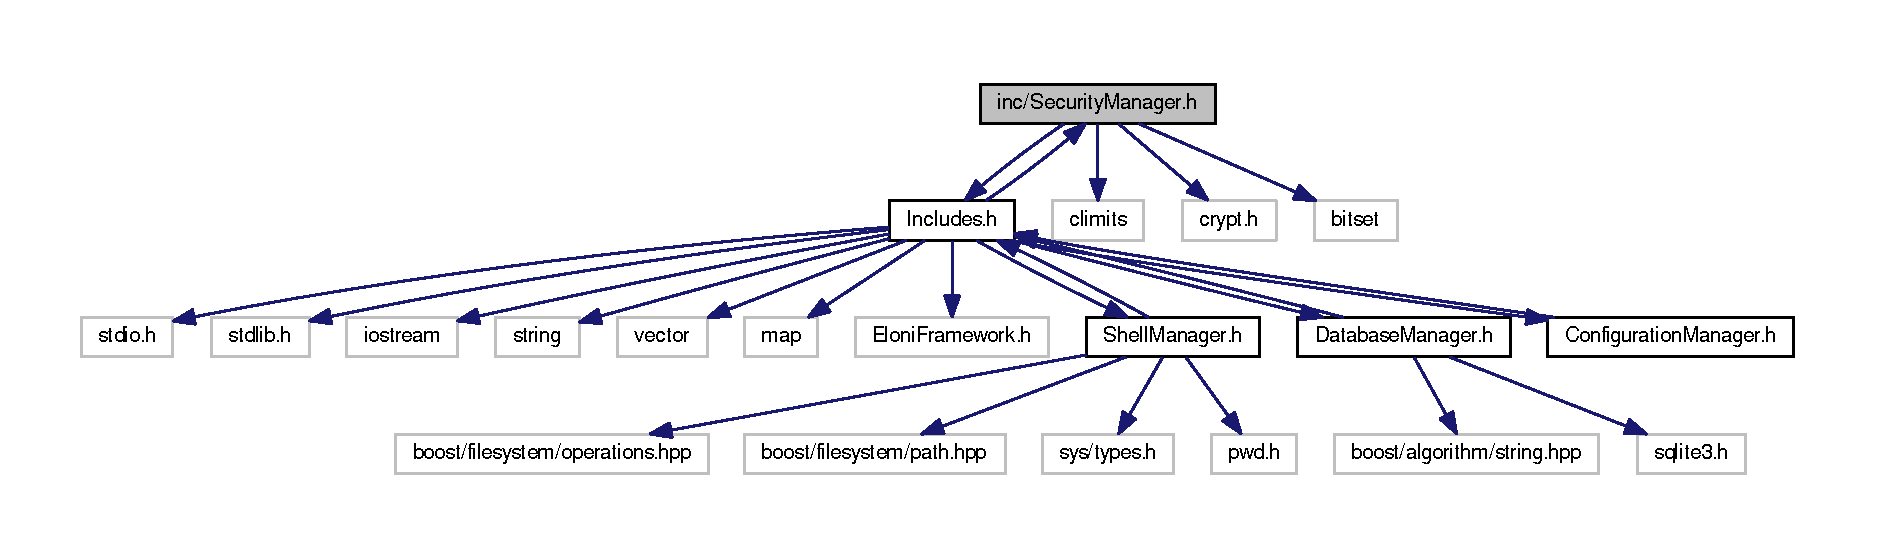
\includegraphics[width=350pt]{SecurityManager_8h__incl}
\end{center}
\end{figure}
This graph shows which files directly or indirectly include this file\-:
\nopagebreak
\begin{figure}[H]
\begin{center}
\leavevmode
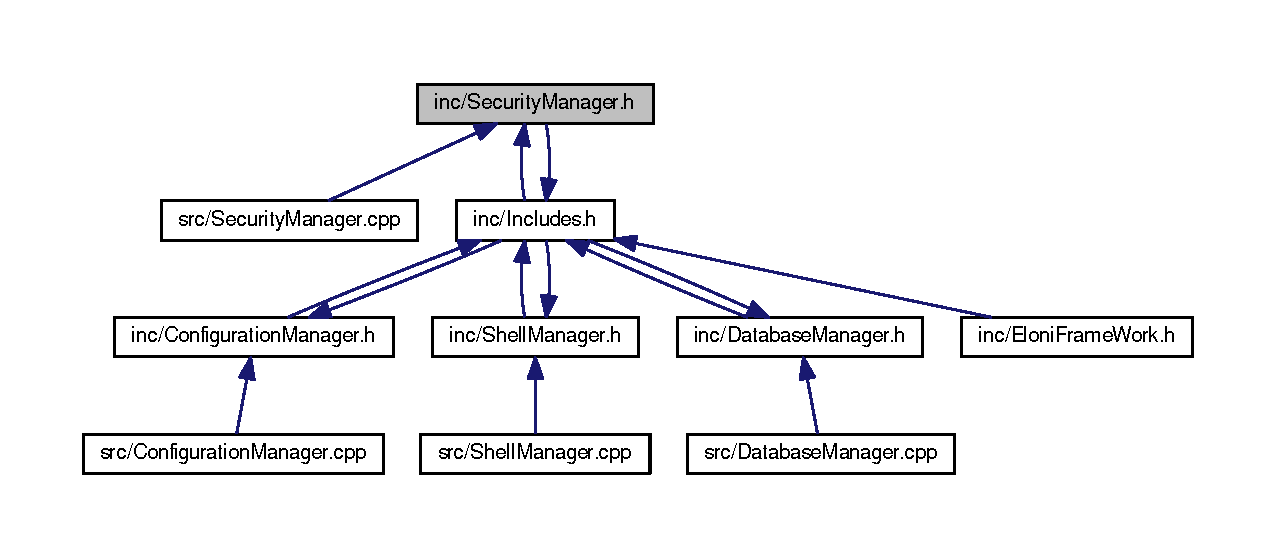
\includegraphics[width=350pt]{SecurityManager_8h__dep__incl}
\end{center}
\end{figure}
\subsection*{Classes}
\begin{DoxyCompactItemize}
\item 
class \hyperlink{classSecurityManager}{Security\-Manager}
\end{DoxyCompactItemize}


\subsection{Detailed Description}
\begin{DoxyAuthor}{Author}
Yme-\/\-Jan Iedema \href{mailto:yj.iedema@gmail.com}{\tt yj.\-iedema@gmail.\-com}
\end{DoxyAuthor}
\hyperlink{classDatabaseManager}{Database\-Manager}

\hyperlink{classSecurityManager}{Security\-Manager}

This class will handle everything related to security extracting users from the database and assigning roles Also allow sertain pages for specific roles 

Definition in file \hyperlink{SecurityManager_8h_source}{Security\-Manager.\-h}.


\hypertarget{SecurityManager_8h}{\section{Security\-Manager.\-h}
\label{SecurityManager_8h}\index{inc/\-Security\-Manager.\-h@{inc/\-Security\-Manager.\-h}}
}

\begin{DoxyCode}
00001 \textcolor{comment}{/**}
00002 \textcolor{comment}{ * @author Yme-Jan Iedema <yj.iedema@gmail.com>}
00003 \textcolor{comment}{ * @file SecurityManager.h}
00004 \textcolor{comment}{ * @dependency DatabaseManager}
00005 \textcolor{comment}{ * }
00006 \textcolor{comment}{ * SecurityManager}
00007 \textcolor{comment}{ * }
00008 \textcolor{comment}{ * This class will handle everything related to security}
00009 \textcolor{comment}{ * extracting users from the database and assigning roles}
00010 \textcolor{comment}{ * Also allow sertain pages for specific roles}
00011 \textcolor{comment}{ * }
00012 \textcolor{comment}{ */}
00013  
00014 \textcolor{preprocessor}{#ifndef DG2\_SECURITYMANAGER\_H}
00015 \textcolor{preprocessor}{}\textcolor{preprocessor}{#define DG2\_SECURITYMANAGER\_H}
00016 \textcolor{preprocessor}{}
00017 \textcolor{preprocessor}{#include "Includes.h"}
00018 
00019 \textcolor{preprocessor}{#include <climits>}
00020 \textcolor{preprocessor}{#include <crypt.h>}
00021 \textcolor{preprocessor}{#include <bitset>}
00022 
\hypertarget{SecurityManager_8h_source_l00023}{}\hyperlink{classSecurityManager}{00023} \textcolor{keyword}{class }\hyperlink{classSecurityManager}{SecurityManager} \{
00024   \textcolor{keyword}{private}:
00025   \textcolor{keyword}{public}:
00026     std::string \hyperlink{classSecurityManager_acc4ef8e7685038735e83e73556a5f510}{Encrypt}(std::string str);
00027     std::map<std::string, int> \hyperlink{classSecurityManager_afe3d50265be58ec179058feadd9902a6}{getRoles}();
00028     \textcolor{keywordtype}{bool} \hyperlink{classSecurityManager_a2950edc6463999ceca399d47023adddc}{hasRole}(std::string username, std::string role);
00029     \textcolor{keywordtype}{void} \hyperlink{classSecurityManager_a9ebf385f13f1893bb36647605677043d}{addRole}(std::string username, std::string role);
00030     \textcolor{keywordtype}{void} \hyperlink{classSecurityManager_a2d5b4923acbe73b0d21c5179deb7f17d}{removeRole}(std::string username, std::string role);
00031     \textcolor{keywordtype}{void} \hyperlink{classSecurityManager_ac9dc2c5a7667b95d9850ff22fc897213}{addUser}(std::string username, std::string password);
00032     \textcolor{keywordtype}{void} \hyperlink{classSecurityManager_ad616d32abdd366d50dfd01091d6a1f0c}{setUser}(std::string username, std::string var, std::string val);
00033     \textcolor{keywordtype}{void} \hyperlink{classSecurityManager_a61db3bbbb21105c441d2a7bc75fb41bd}{deleteUser}(std::string username);
00034     \textcolor{keywordtype}{bool} \hyperlink{classSecurityManager_abda859f83e39977a46ce993970a35f92}{isUser}(std::string username);
00035     std::vector<std::string> \hyperlink{classSecurityManager_a05f3c7fc498871277a00dffa092614c1}{getUsers}();
00036     \textcolor{keywordtype}{bool} \hyperlink{classSecurityManager_ace68188567f645c18097b8791db64b41}{Authenticate}(std::string username, std::string password);
00037 \};
00038 
00039 \textcolor{preprocessor}{#endif}
\end{DoxyCode}

\hypertarget{ShellManager_8h}{\section{inc/\-Shell\-Manager.h File Reference}
\label{ShellManager_8h}\index{inc/\-Shell\-Manager.\-h@{inc/\-Shell\-Manager.\-h}}
}
{\ttfamily \#include \char`\"{}Includes.\-h\char`\"{}}\\*
{\ttfamily \#include $<$boost/filesystem/operations.\-hpp$>$}\\*
{\ttfamily \#include $<$boost/filesystem/path.\-hpp$>$}\\*
{\ttfamily \#include $<$sys/types.\-h$>$}\\*
{\ttfamily \#include $<$pwd.\-h$>$}\\*
Include dependency graph for Shell\-Manager.\-h\-:
\nopagebreak
\begin{figure}[H]
\begin{center}
\leavevmode
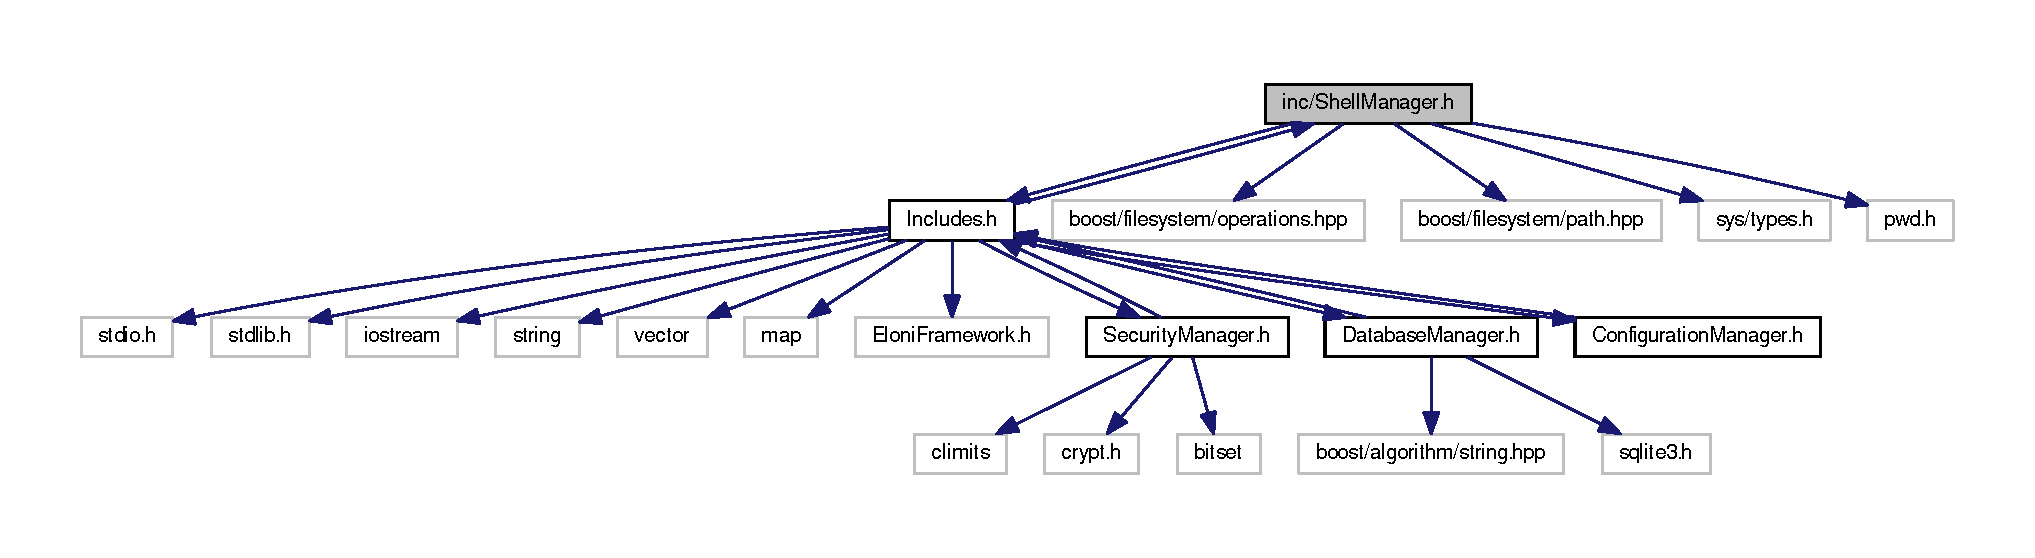
\includegraphics[width=350pt]{ShellManager_8h__incl}
\end{center}
\end{figure}
This graph shows which files directly or indirectly include this file\-:
\nopagebreak
\begin{figure}[H]
\begin{center}
\leavevmode
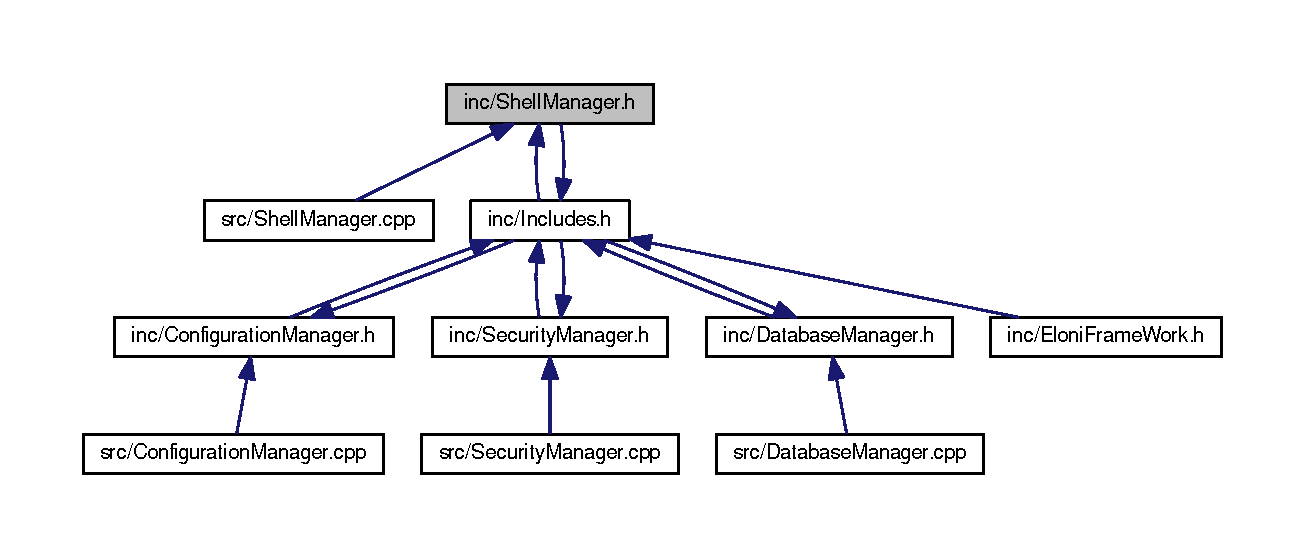
\includegraphics[width=350pt]{ShellManager_8h__dep__incl}
\end{center}
\end{figure}
\subsection*{Classes}
\begin{DoxyCompactItemize}
\item 
class \hyperlink{classShellManager}{Shell\-Manager}
\end{DoxyCompactItemize}


\subsection{Detailed Description}
\begin{DoxyAuthor}{Author}
Yme-\/\-Jan Iedema \href{mailto:yj.iedema@gmail.com}{\tt yj.\-iedema@gmail.\-com}
\end{DoxyAuthor}
\hyperlink{classShellManager}{Shell\-Manager}

This class will allow the usage of 'some' bash commands ran as a specific user. 

Definition in file \hyperlink{ShellManager_8h_source}{Shell\-Manager.\-h}.


\hypertarget{ShellManager_8h}{\section{Shell\-Manager.\-h}
\label{ShellManager_8h}\index{inc/\-Shell\-Manager.\-h@{inc/\-Shell\-Manager.\-h}}
}

\begin{DoxyCode}
00001 \textcolor{comment}{/**}
00002 \textcolor{comment}{ * @author Yme-Jan Iedema <yj.iedema@gmail.com>}
00003 \textcolor{comment}{ * @file ShellManager.h}
00004 \textcolor{comment}{ * }
00005 \textcolor{comment}{ * ShellManager}
00006 \textcolor{comment}{ * }
00007 \textcolor{comment}{ * This class will allow the usage of 'some' bash commands ran as a }
00008 \textcolor{comment}{ * specific user.}
00009 \textcolor{comment}{ */}
00010 
00011 \textcolor{preprocessor}{#ifndef DG2\_BASHMANAGER\_H}
00012 \textcolor{preprocessor}{}\textcolor{preprocessor}{#define DG2\_BASHMANAGER\_H}
00013 \textcolor{preprocessor}{}
00014 \textcolor{comment}{// Include all general headers}
00015 \textcolor{preprocessor}{#include "Includes.h"}
00016 
00017 \textcolor{comment}{// Class specific headers}
00018 \textcolor{preprocessor}{#include <boost/filesystem/operations.hpp>}
00019 \textcolor{preprocessor}{#include <boost/filesystem/path.hpp>}
00020 \textcolor{preprocessor}{#include <sys/types.h>}
00021 \textcolor{preprocessor}{#include <pwd.h>}
00022 
00023 \textcolor{keyword}{namespace }fs = boost::filesystem;
00024 
\hypertarget{ShellManager_8h_source_l00025}{}\hyperlink{classShellManager}{00025} \textcolor{keyword}{class }\hyperlink{classShellManager}{ShellManager} \{
00026   \textcolor{keyword}{private}:
00027     \textcolor{keyword}{struct }passwd             pwd;
00028     \textcolor{keyword}{struct }passwd             *result;
00029     \textcolor{keywordtype}{char}                      *buf;
00030     \textcolor{keywordtype}{size\_t}                    bufsize;
00031     \textcolor{keywordtype}{int}                       s;
00032     std::string               \_dir;
00033     uid\_t                     ruid, euid, saveduid;
00034     std::vector<std::string>  blacklist;
00035     
00036   \textcolor{keyword}{public}:
00037     \hyperlink{classShellManager_a04dec3699269bb388648f6017fd9fd15}{ShellManager}();
00038     \textcolor{keywordtype}{int}           \hyperlink{classShellManager_a9e595c79f89d7c796df213b469384e08}{setUser}(std::string Username);
00039     \textcolor{keywordtype}{int}           \hyperlink{classShellManager_a9e595c79f89d7c796df213b469384e08}{setUser}(\textcolor{keywordtype}{int} UserID);
00040     std::string   \hyperlink{classShellManager_aeed1b234a317e951f01bdc42a2097d40}{setWorkingDirectory}(std::string dir);
00041     std::string   \hyperlink{classShellManager_a9f40b1296bef8f0d694cafdca29e0e13}{Execute}(std::string cmd);
00042 \};
00043 
00044 \textcolor{preprocessor}{#endif}
\end{DoxyCode}

%--- End generated contents ---

% Index
\newpage
\phantomsection
\addcontentsline{toc}{chapter}{Index}
\printindex

\end{document}
